% This must be in the first 5 lines to tell arXiv to use pdfLaTeX, which is strongly recommended.
\pdfoutput=1
% In particular, the hyperref package requires pdfLaTeX in order to break URLs across lines.

\documentclass[11pt]{article}

% Remove the "review" option to generate the final version.
\usepackage{acl}

% Standard package includes
\usepackage{times}
\usepackage{latexsym}

% For proper rendering and hyphenation of words containing Latin characters (including in bib files)
\usepackage[T1]{fontenc}
% For Vietnamese characters
% \usepackage[T5]{fontenc}
% See https://www.latex-project.org/help/documentation/encguide.pdf for other character sets

% This assumes your files are encoded as UTF8
\usepackage[utf8]{inputenc}

% This is not strictly necessary, and may be commented out,
% but it will improve the layout of the manuscript,
% and will typically save some space.
\usepackage{microtype}

\usepackage{graphicx}
\graphicspath{ {../images/} }

% If the title and author information does not fit in the area allocated, uncomment the following
%
%\setlength\titlebox{<dim>}
%
% and set <dim> to something 5cm or larger.

\title{Détermination du parti politique auquel appartient l’orateur}

% Author information can be set in various styles:
% For several authors from the same institution:
% \author{Author 1 \and ... \and Author n \\
%         Address line \\ ... \\ Address line}
% if the names do not fit well on one line use
%         Author 1 \\ {\bf Author 2} \\ ... \\ {\bf Author n} \\
% For authors from different institutions:
% \author{Author 1 \\ Address line \\  ... \\ Address line
%         \And  ... \And
%         Author n \\ Address line \\ ... \\ Address line}
% To start a seperate ``row'' of authors use \AND, as in
% \author{Author 1 \\ Address line \\  ... \\ Address line
%         \AND
%         Author 2 \\ Address line \\ ... \\ Address line \And
%         Author 3 \\ Address line \\ ... \\ Address line}

\author{Eve Sauvage \\
  Université Paris Nanterre \\
  \texttt{41017970@parisnanterre.fr}}

\begin{document}
\maketitle
\begin{abstract}
Ce document explore l'analyse d'opinion à partir d'un corpus regroupant un ensemble de débats au Parlement européen en trois langues, le français, l'anglais et l'italien. L'objectif de la tâche est d'assigner correctement les partis politiques aux interventions des parlementaires. Nous utiliserons pour cela plusieurs modèles d'apprentissage artificiel afin de déterminer un modèle idéal.
\end{abstract}

\section{Introduction}

\subparagraph{}
La tâche visée par ce document est proposée par l'édition 2009 du défi fouille de texte organisé par l'université Paris Saclay. Cette édition se concentre sur l'analyse d'opinion multilingue et notamment en explorant l'affectation des interventions au parlement européen à des partis politiques. Les corpus utilisés pour l'entraînement et la vérification des modèles sont fournis en français, anglais et italien.
\subparagraph{}
Dans nos expériences, on suppose que la différences entre les langues nécessite que les modèles soient entraînés séparemments. Nous chercherons d'abord à déterminer le meilleur modèle sur le français avant d'essayer d'observer son efficacité sur l'anglais et l'italien. Le modèle choisi sera réentraîné sur les langues en question pour une plus grande adaptabilité.

\section{Traitement des données}

\subparagraph{}
Les fichiers de corpus sont disponibles au format xml ce qui permet de récupérer aisement leur contenu à l'aide de la bibliothèque python \texttt{xml.etree.ElementTree} qui permet d'accéder directement aux noeuds du fichier grâce à leur nom. Les données d'entraînement sont séparées en deux listes ordonnées contenant le texte d'un côté et les étiquettes correspondantes de l'autre.
\subparagraph{}
Nous decidons d'entraîner le modèle sur la totalité des données d'entraînement et de récupérer les annotations de référence pour vérifier nos résultats. Les deux nouvelles listes obtenues sont nettoyées des résultats vides afin d'éviter les erreurs lors du décompte des résultats.
\subparagraph{}
Dans un premier temps, nous realiserons la vectorisation du texte à l'aide du TF-IDF proposé par la bibliothèque \texttt{scikit-learn} sans lemmatisation du texte d'origine. Nous réviserons cette approche au vu des résultats.

\section{Résultats}

\subsection{Arbres de décisions}

\subparagraph{}
Nous entraînons d'abord les données à l'aide d'un modèle d'arbre de décision : un modèle simple et permettant une visualisation. Ce premier modèle simple constitura notre modèle baseline avec lequel nous comparerons nos prochains essais.

\begin{table}[h]
\centering
\begin{tabular}{lcccc}
\hline
 & precision & recall & f-score & support\\
\hline
ELDR & 0.72 & 0.67 & 0.70 & 1339\\
GUE-NGL & 0.75 & 0.75 & 0.75 & 1793\\
PPE-DE & 0.76 & 0.78 & 0.77 & 4571\\ 
PSE &  0.73 & 0.73 & 0.73 & 3627\\ 
Verts-ALE & 0.69 & 0.67 & 0.68 & 1585\\
\hline
accuracy& & & 0.74 & 12917\\
macro avg & 0.73 & 0.72 & 0.73& 12917\\
weighted avg & 0.74 & 0.74 & 0.74& 12917\\
\hline
\end{tabular}
\caption{rapport de classification pour le modèle arbre de décision}
\label{tab:accents}
\end{table}

\begin{figure}[h]
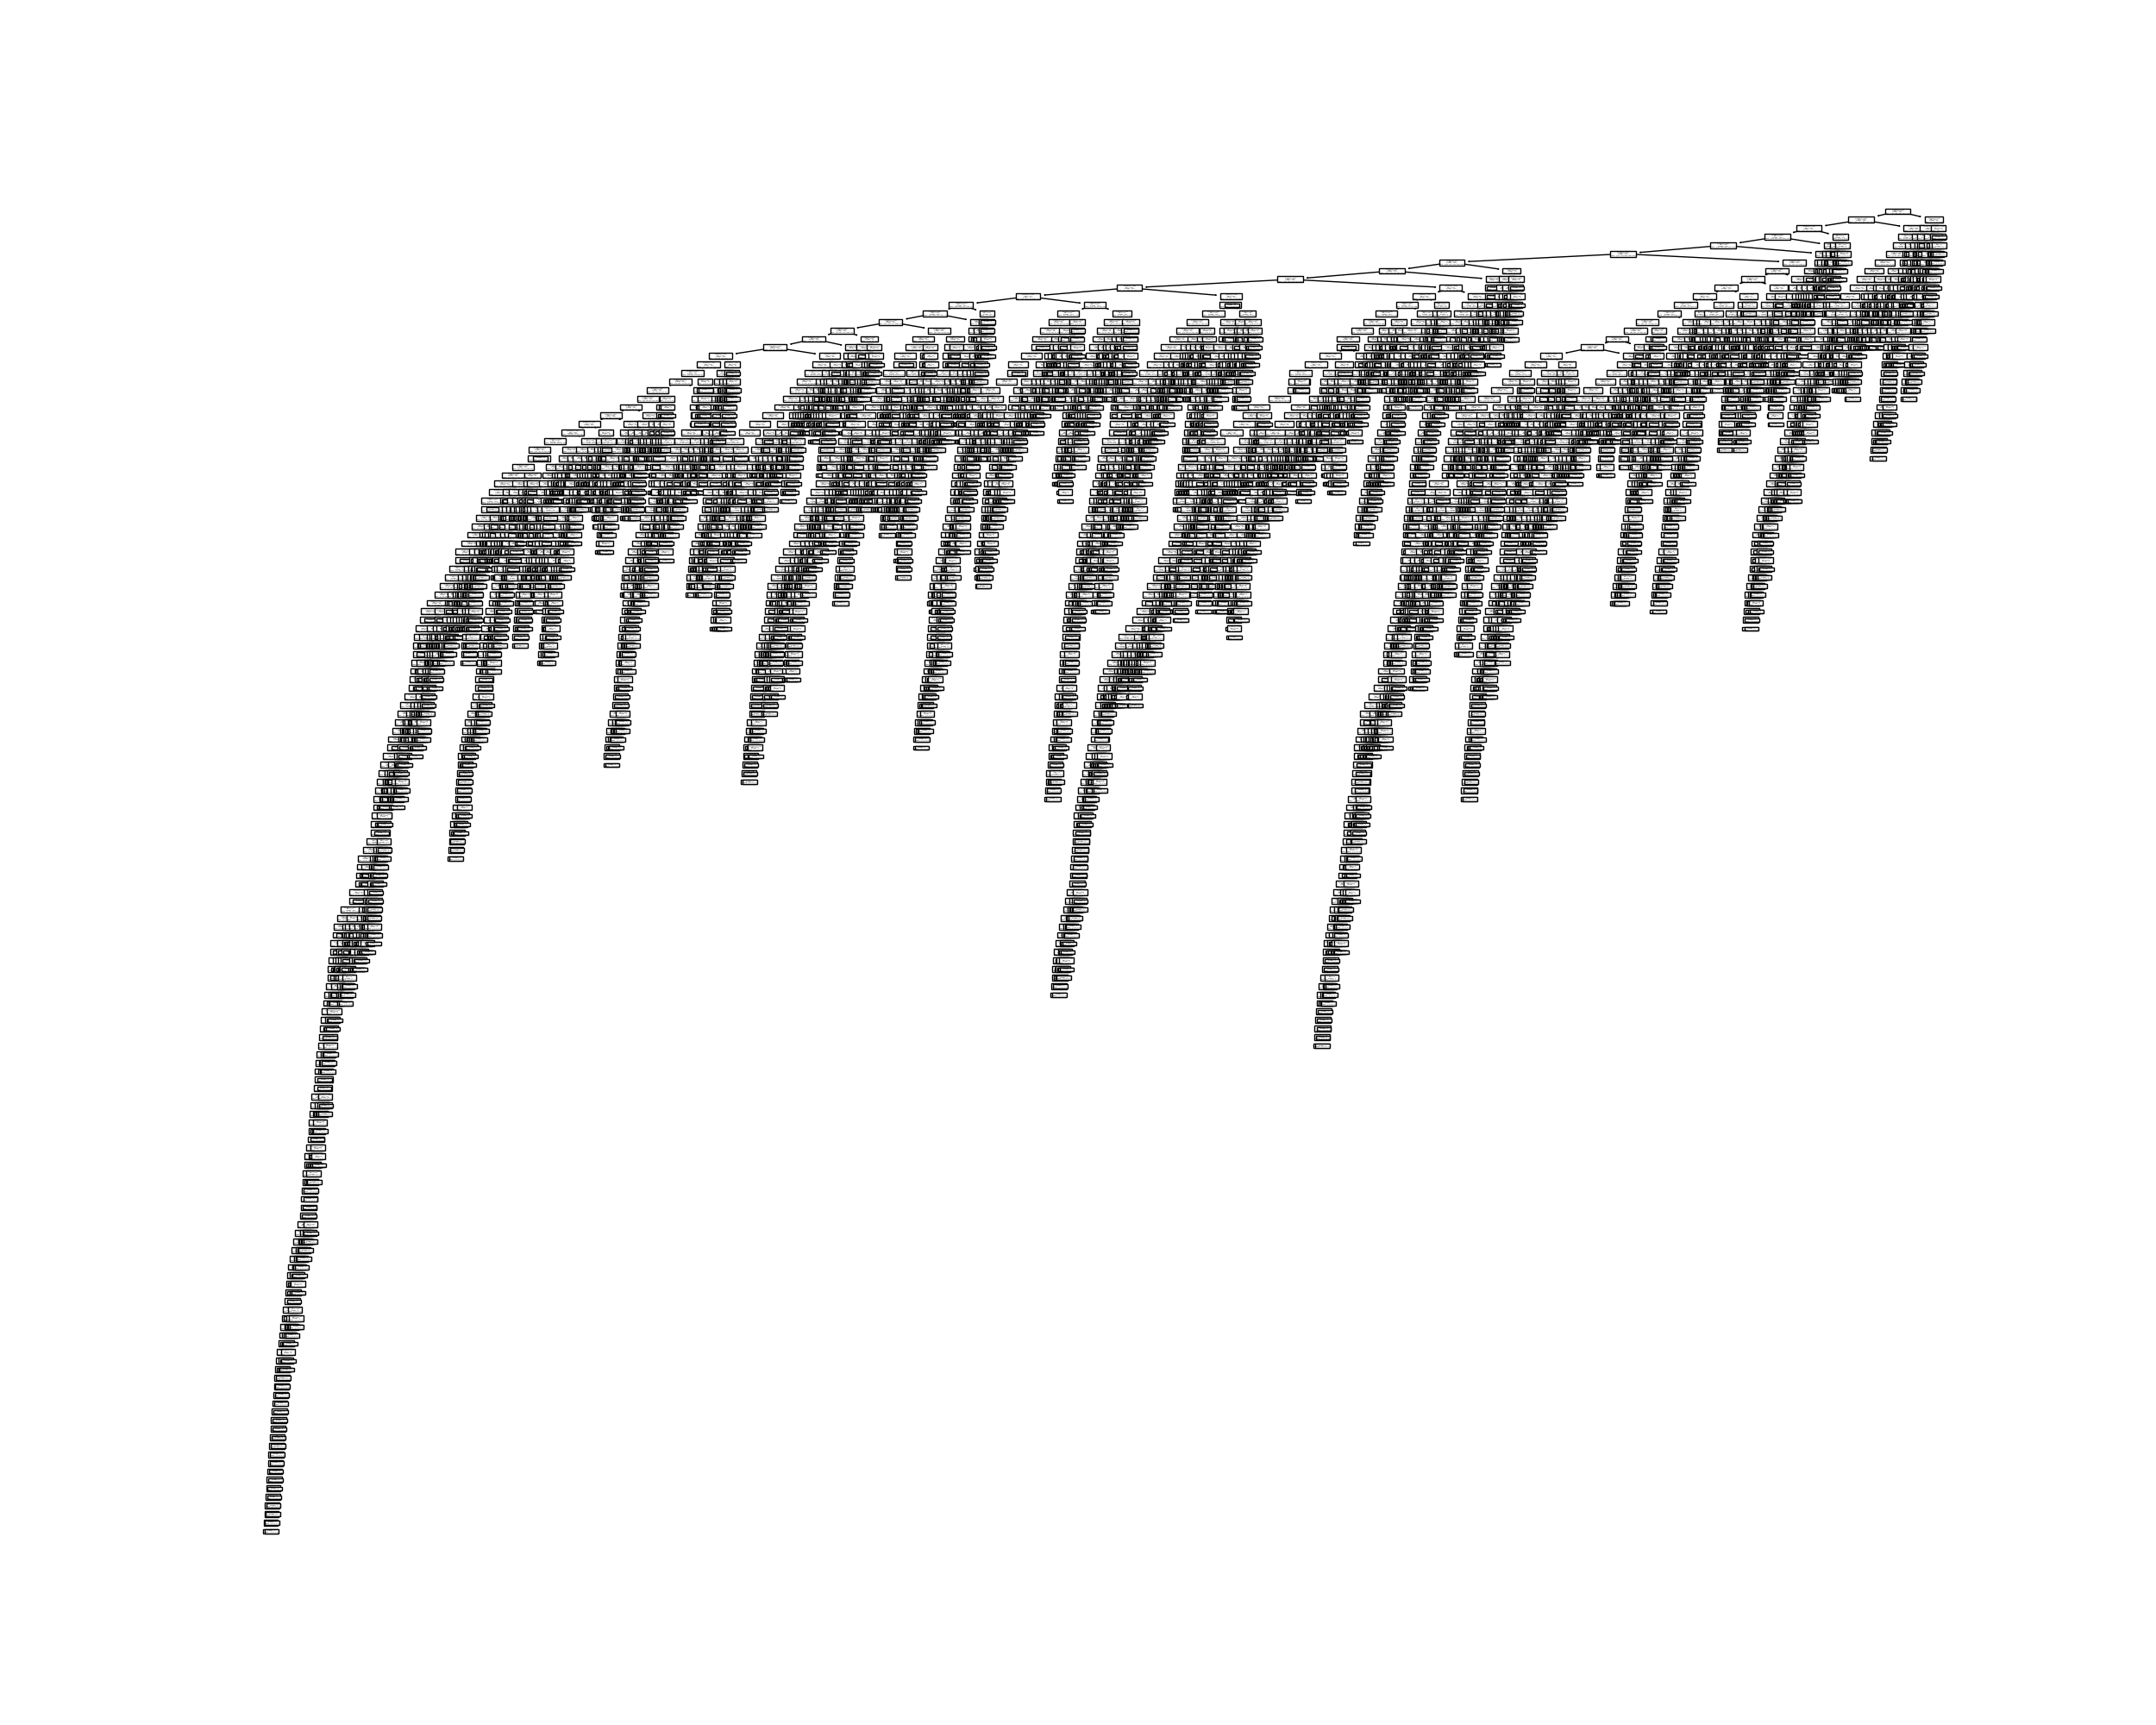
\includegraphics[width=0.5\textwidth]{decision_tree}
\caption{représentation du modèle}
\centering
\end{figure}

\begin{figure}[h]
\includegraphics[width=0.5\textwidth]{MatriceConfusionTree}
\caption{Matrice de confusion pour l'arbre de décision}
\centering
\end{figure}

\subparagraph{}
Les résultats obtenus sont satisfaisants étant donné la difficulté de la tâche et les résultats d'annotation manuelle présentées par (Groin, 2009). Toutefois, il semble, en visualisant l'arbre de décision obtenu, que le modèle surapprend les données fournies. Ce surapprentissage est lié à l'absence de restriction de profondeur ainsi qu'à la multiplicité des paramètres entaîné par l'utilisation d'un TF-IDF pour la vectorisation des données. Il est donc pertinent de réduire le nombre de paramètres pour utiliser pleinement le potentiel de visualisation du modèle.
\subsubsection{lemmatisation et suppression des mots stops}
Nous supposons que la suppression de la ponctuation ainsi que sa lemmatisation et la suppression des mots stops amélioreront la profondeur du modèle d'arbre de décision. Toutefois, les expériences montrent que les résultats se détériorent et que la profondeur augmente. 
\subsubsection{Réequilibrage des données}
\subparagraph{}
On essaie également de réequilibrer les données d'entrainement afin de supprimer le biais du modèle mais si la précision et le rappel s'améliorent dans les classes minoritaires, les très mauvais résultats dans les classes réequilibrées nous invite à conserver le biais de départ afin de conserver une f-mesure acceptable. Les mauvais résultats dans les classes majoritaires persistent lorsque l'on rééquilibre également les données de tests. En revanche, le rééquilibrage des données permet d'effectivement diminuer la profondeur de l'arbre en utilisant un rééquilibrage par downsampling en passant d'un profondeur de 146 à une prodondeur de 96 grâce au downsampling.

\begin{figure}[h]
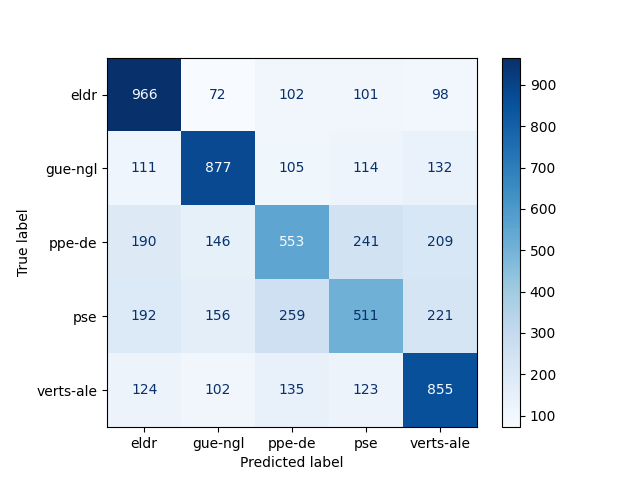
\includegraphics[width=0.5\textwidth]{matriceConfusionTreeBalanced}
\caption{Matrice de confusion avec apprentissage sur des données rééquilibrées en downsampling}
\centering
\end{figure}

\subparagraph{}
Le upsampling permet de moins déteriorer les résultats pour les classes précédemment majoritaire et diminue de ce fait, moins le résultat général. Le modèle entraîné avec le réequilibrage en upsampling présente une f mesure moyenne de 0.65.

\subsection{Random Forest}
Face à ces résultats peu fructueux, nous essayons d'autres modèles d'apprentissage en commençant par Random Forest qui devrait présenter de meilleurs résultats. En effet, le modèle Random Forest permet de combiner plusieurs arbres de décisions augmentant ainsi leur efficacité.


\begin{table}[h]
\centering
\begin{tabular}{lccc}
\hline
 & precision & recall & f-score\\
\hline
ELDR & 1.00 & 0.61 & 0.76\\
GUE-NGL& 0.97 &0.71 & 0.82\\
PPE-DE & 0.64 &0.95 & 0.76\\ 
PSE &  0.83&  0.69 & 0.75\\ 
Verts-ALE &  1.00 & 0.61& 0.76\\
\hline
accuracy& & &    0.77 \\
macro avg &  0.89 &  0.71 &  0.77 \\
weighted avg &  0.82 & 0.77  &  0.77  \\
\hline
\end{tabular}
\caption{rapport de classification pour le modèle random forest sans pretraitement}
\label{tab:accents}
\end{table}

\subparagraph{}
La f-mesure moyenne de random Forest sans modification des données est effectivement meilleure que celle des arbres de décisions testés précedemment avec un score de 77\%. Toutefois, la progression est médiocre, l'augmentation n'étant que d'2\%.
\subparagraph{}
Dans le cas de random Forest, la simplification des données semble avoir moins d'impact en particulier dans le cas de la lemmatisation qui ne fait perdre aucun point à la f-mesure moyenne.

\subsection{LinearSVC}
\subparagraph{}
On arrive à augmenter le score grâce à un modèle de Classification par Support de Vecteur linéaire.

\begin{quote}
\begin{verbatim}
\documentclass[11pt]{article}
\end{verbatim}
\end{quote}

To load the style file in the review version:
\begin{quote}
\begin{verbatim}
\usepackage[review]{acl}
\end{verbatim}
\end{quote}
For the final version, omit the \verb|review| option:
\begin{quote}
\begin{verbatim}
\usepackage{acl}
\end{verbatim}
\end{quote}

To use Times Roman, put the following in the preamble:
\begin{quote}
\begin{verbatim}
\usepackage{times}
\end{verbatim}
\end{quote}
(Alternatives like txfonts or newtx are also acceptable.)

Please see the \LaTeX{} source of this document for comments on other packages that may be useful.

Set the title and author using \verb|\title| and \verb|\author|. Within the author list, format multiple authors using \verb|\and| and \verb|\And| and \verb|\AND|; please see the \LaTeX{} source for examples.

By default, the box containing the title and author names is set to the minimum of 5 cm. If you need more space, include the following in the preamble:
\begin{quote}
\begin{verbatim}
\setlength\titlebox{<dim>}
\end{verbatim}
\end{quote}
where \verb|<dim>| is replaced with a length. Do not set this length smaller than 5 cm.

\section{Document Body}

\subsection{Footnotes}

Footnotes are inserted with the \verb|\footnote| command.\footnote{This is a footnote.}

\subsection{Tables and figures}

See Table~\ref{tab:accents} for an example of a table and its caption.
\textbf{Do not override the default caption sizes.}

\begin{table}
\centering
\begin{tabular}{lc}
\hline
\textbf{Command} & \textbf{Output}\\
\hline
\verb|{\"a}| & {\"a} \\
\verb|{\^e}| & {\^e} \\
\verb|{\`i}| & {\`i} \\ 
\verb|{\.I}| & {\.I} \\ 
\verb|{\o}| & {\o} \\
\verb|{\'u}| & {\'u}  \\ 
\verb|{\aa}| & {\aa}  \\\hline
\end{tabular}
\begin{tabular}{lc}
\hline
\textbf{Command} & \textbf{Output}\\
\hline
\verb|{\c c}| & {\c c} \\ 
\verb|{\u g}| & {\u g} \\ 
\verb|{\l}| & {\l} \\ 
\verb|{\~n}| & {\~n} \\ 
\verb|{\H o}| & {\H o} \\ 
\verb|{\v r}| & {\v r} \\ 
\verb|{\ss}| & {\ss} \\
\hline
\end{tabular}
\caption{Example commands for accented characters, to be used in, \emph{e.g.}, Bib\TeX{} entries.}
\label{tab:accents}
\end{table}

\subsection{Hyperlinks}

Users of older versions of \LaTeX{} may encounter the following error during compilation: 
\begin{quote}
\tt\verb|\pdfendlink| ended up in different nesting level than \verb|\pdfstartlink|.
\end{quote}
This happens when pdf\LaTeX{} is used and a citation splits across a page boundary. The best way to fix this is to upgrade \LaTeX{} to 2018-12-01 or later.

\subsection{Citations}

\begin{table*}
\centering
\begin{tabular}{lll}
\hline
\textbf{Output} & \textbf{natbib command} & \textbf{Old ACL-style command}\\
\hline
\citep{Gusfield:97} & \verb|\citep| & \verb|\cite| \\
\citealp{Gusfield:97} & \verb|\citealp| & no equivalent \\
\citet{Gusfield:97} & \verb|\citet| & \verb|\newcite| \\
\citeyearpar{Gusfield:97} & \verb|\citeyearpar| & \verb|\shortcite| \\
\hline
\end{tabular}
\caption{\label{citation-guide}
Citation commands supported by the style file.
The style is based on the natbib package and supports all natbib citation commands.
It also supports commands defined in previous ACL style files for compatibility.
}
\end{table*}

Table~\ref{citation-guide} shows the syntax supported by the style files.
We encourage you to use the natbib styles.
You can use the command \verb|\citet| (cite in text) to get ``author (year)'' citations, like this citation to a paper by \citet{Gusfield:97}.
You can use the command \verb|\citep| (cite in parentheses) to get ``(author, year)'' citations \citep{Gusfield:97}.
You can use the command \verb|\citealp| (alternative cite without parentheses) to get ``author, year'' citations, which is useful for using citations within parentheses (e.g. \citealp{Gusfield:97}).

\subsection{References}

\nocite{Ando2005,andrew2007scalable,rasooli-tetrault-2015}

The \LaTeX{} and Bib\TeX{} style files provided roughly follow the American Psychological Association format.
If your own bib file is named \texttt{custom.bib}, then placing the following before any appendices in your \LaTeX{} file will generate the references section for you:
\begin{quote}
\begin{verbatim}
\bibliography{custom}
\end{verbatim}
\end{quote}

You can obtain the complete ACL Anthology as a Bib\TeX{} file from \url{https://aclweb.org/anthology/anthology.bib.gz}.
To include both the Anthology and your own .bib file, use the following instead of the above.
\begin{quote}
\begin{verbatim}
\bibliography{anthology,custom}
\end{verbatim}
\end{quote}

Please see Section~\ref{sec:bibtex} for information on preparing Bib\TeX{} files.

\subsection{Appendices}

Use \verb|\appendix| before any appendix section to switch the section numbering over to letters. See Appendix~\ref{sec:appendix} for an example.

\section{Bib\TeX{} Files}
\label{sec:bibtex}

Unicode cannot be used in Bib\TeX{} entries, and some ways of typing special characters can disrupt Bib\TeX's alphabetization. The recommended way of typing special characters is shown in Table~\ref{tab:accents}.

Please ensure that Bib\TeX{} records contain DOIs or URLs when possible, and for all the ACL materials that you reference.
Use the \verb|doi| field for DOIs and the \verb|url| field for URLs.
If a Bib\TeX{} entry has a URL or DOI field, the paper title in the references section will appear as a hyperlink to the paper, using the hyperref \LaTeX{} package.

\section*{Acknowledgements}

This document has been adapted
by Steven Bethard, Ryan Cotterell and Rui Yan
from the instructions for earlier ACL and NAACL proceedings, including those for 
ACL 2019 by Douwe Kiela and Ivan Vuli\'{c},
NAACL 2019 by Stephanie Lukin and Alla Roskovskaya, 
ACL 2018 by Shay Cohen, Kevin Gimpel, and Wei Lu, 
NAACL 2018 by Margaret Mitchell and Stephanie Lukin,
Bib\TeX{} suggestions for (NA)ACL 2017/2018 from Jason Eisner,
ACL 2017 by Dan Gildea and Min-Yen Kan, 
NAACL 2017 by Margaret Mitchell, 
ACL 2012 by Maggie Li and Michael White, 
ACL 2010 by Jing-Shin Chang and Philipp Koehn, 
ACL 2008 by Johanna D. Moore, Simone Teufel, James Allan, and Sadaoki Furui, 
ACL 2005 by Hwee Tou Ng and Kemal Oflazer, 
ACL 2002 by Eugene Charniak and Dekang Lin, 
and earlier ACL and EACL formats written by several people, including
John Chen, Henry S. Thompson and Donald Walker.
Additional elements were taken from the formatting instructions of the \emph{International Joint Conference on Artificial Intelligence} and the \emph{Conference on Computer Vision and Pattern Recognition}.

% Entries for the entire Anthology, followed by custom entries
\bibliography{anthology,custom}

\appendix

\section{Example Appendix}
\label{sec:appendix}

This is an appendix.

\end{document}
